%%%%%%%%%%%%%%%%%%%%%%%%%%%%%%%%%%%%%%%%%
% Short Sectioned Assignment
% LaTeX Template
% Version 1.0 (5/5/12)
%
% This template has been downloaded from:
% http://www.LaTeXTemplates.com
%
% Original author:
% Frits Wenneker (http://www.howtotex.com)
%
% License:
% CC BY-NC-SA 3.0 (http://creativecommons.org/licenses/by-nc-sa/3.0/)
%
%%%%%%%%%%%%%%%%%%%%%%%%%%%%%%%%%%%%%%%%%

%----------------------------------------------------------------------------------------
%	PACKAGES AND OTHER DOCUMENT CONFIGURATIONS
%----------------------------------------------------------------------------------------

\documentclass[paper=a4, fontsize=12pt]{scrartcl} % A4 paper and 11pt font size

\usepackage[T1]{fontenc} % Use 8-bit encoding that has 256 glyphs
\usepackage{fourier} % Use the Adobe Utopia font for the document - comment this line to return to the LaTeX default
\usepackage[english]{babel} % English language/hyphenation
\usepackage{amsmath,amsfonts,amsthm} % Math packages

\usepackage{graphicx}
\usepackage{extarrows}
\usepackage{amssymb}
\usepackage{bm}


\usepackage{lipsum} % Used for inserting dummy 'Lorem ipsum' text into the template

\usepackage{sectsty} % Allows customizing section commands
\allsectionsfont{\centering \normalfont\scshape} % Make all sections centered, the default font and small caps

\usepackage{fancyhdr} % Custom headers and footers
\pagestyle{fancyplain} % Makes all pages in the document conform to the custom headers and footers
\fancyhead{} % No page header - if you want one, create it in the same way as the footers below
\fancyfoot[L]{} % Empty left footer
\fancyfoot[C]{} % Empty center footer
\fancyfoot[R]{\thepage} % Page numbering for right footer
\renewcommand{\headrulewidth}{0pt} % Remove header underlines
\renewcommand{\footrulewidth}{0pt} % Remove footer underlines
\setlength{\headheight}{13.6pt} % Customize the height of the header

\numberwithin{equation}{section} % Number equations within sections (i.e. 1.1, 1.2, 2.1, 2.2 instead of 1, 2, 3, 4)
\numberwithin{figure}{section} % Number figures within sections (i.e. 1.1, 1.2, 2.1, 2.2 instead of 1, 2, 3, 4)
\numberwithin{table}{section} % Number tables within sections (i.e. 1.1, 1.2, 2.1, 2.2 instead of 1, 2, 3, 4)

\setlength\parindent{0pt} % Removes all indentation from paragraphs - comment this line for an assignment with lots of text

%----------------------------------------------------------------------------------------
%	TITLE SECTION
%----------------------------------------------------------------------------------------

\newcommand{\horrule}[1]{\rule{\linewidth}{#1}} % Create horizontal rule command with 1 argument of height

\title{	
\normalfont \normalsize 
\textsc{National Sun Yat-sen University, Department of Mathematics} \\ [25pt] % Your university, school and/or department name(s)
\horrule{0.5pt} \\[0.4cm] % Thin top horizontal rule
\huge Reliability Analysis Assignment 5 \\(personal)\\ % The assignment title
\horrule{2pt} \\[0.5cm] % Thick bottom horizontal rule
}

\author{Kuan-I Chung} % Your name

\date{\normalsize 2017.06.23} % Today's date or a custom date

\begin{document}

\maketitle % Print the title

%----------------------------------------------------------------------------------------
%	7.6
%----------------------------------------------------------------------------------------
7.6
\begin{itemize}
	\item[(a)] 	\ \\ 
			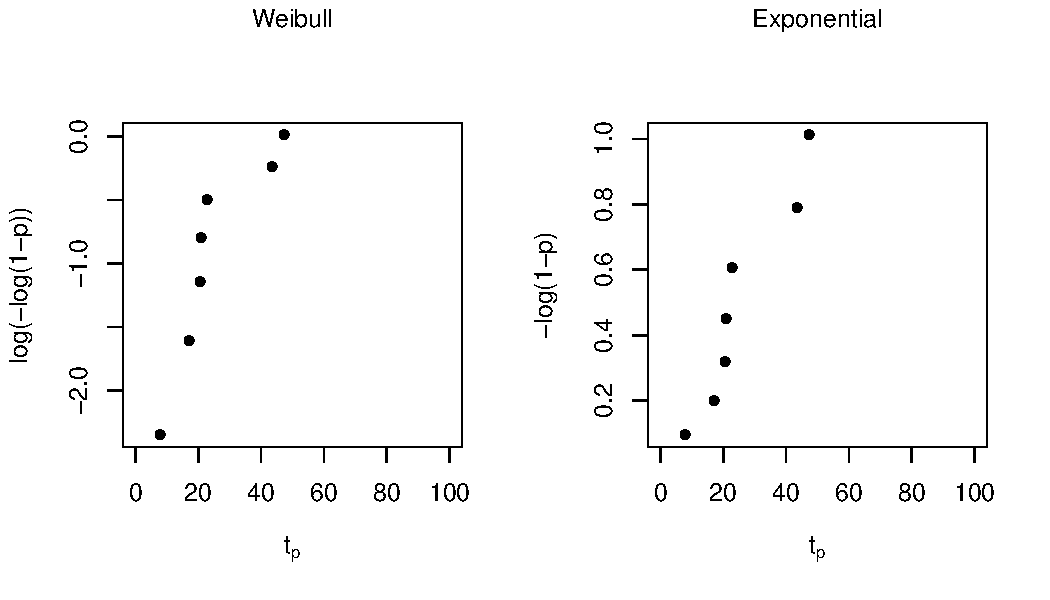
\includegraphics[width = \textwidth]{fig_7_6_a.pdf}
	\item[(b)] 	The exponential probability plot fits better than the Weibull one.
	\item[(c)] 	Let $X_{(1)}, ..., X_{(r)}$ be the exact-timed data and $X_{(r+1)}, ..., X_{(n)}$ be the right censored data. Assume both set of data have exponential distributions with $\theta$, then
			\begin{align*}
				&L(\theta) 		=	\left( \prod_{i = 1}^{r}\frac{1}{\theta}e^{-\frac{x_{(i)}}{\theta}}\right)\left( \prod_{i = r+1}^{n}\frac{1}{\theta}e^{-\frac{x_{(i)}}{\theta}}\right) = \left( \frac{1}{\theta}\right)^re^{-\frac{\sum_{i=1}^nx_{(i)}}{\theta}} = \left( \frac{1}{\theta}\right)^re^{-\frac{\sum_{i=1}^nx_{i}}{\theta}}\\
				\Rightarrow \ \	&log L(\theta) 	=	log \left( \frac{1}{\theta}\right)^r - \frac{\sum_{i=1}^nx_{i}}{\theta} \\
				\text{Let} \ \ \	&\frac{\partial log L(\theta)}{\partial \theta} = -\frac{r}{\theta} +\frac{\sum_{i = 1}^nx_{i}}{\theta^2} = 0\ \Rightarrow \ \widehat{\theta} = \frac{\sum_{i = 1}^nx_{i}}{r}\\
				\because	\ \ &\left. \frac{\partial^2 log L(\theta)}{\partial \theta^2} \right|_{\theta = \widehat{\theta}} = \frac{\sum_{i = 1}^nx_{i} - 2\sum_{i = 1}^nx_{i}}{\theta^3} < 0\\
				\therefore\ \ & \widehat{\theta}_{mle} = \frac{\sum_{i = 1}^nx_{i}}{r}\approx 82.8\\
				\Rightarrow \ \	& Var\left(\widehat{\theta}_{mle}\right) = Var\left(\frac{\sum_{i = 1}^nx_{i}}{r}\right) = Var\left( \frac{2\cdot\frac{\sum_{i = 1}^nx_{i}}{\theta}\cdot\frac{\theta}{2}}{r} \right) \\
				\because\ \ & 2\cdot\frac{\sum_{i = 1}^nx_{i}}{\theta} \sim \chi_{2r}^2 \\
				\Rightarrow \ \	& Var\left(\widehat{\theta}_{mle}\right) = \frac{\theta^2}{4r^2}\cdot 4r = \frac{\theta^2}{r}\\
				\Rightarrow \ \	& se_{\widehat{\theta}_{mle}} = \frac{\theta}{\sqrt{r}} \\
				\Rightarrow \ \	& \widehat{se}_{\widehat{\theta}_{mle}} =  \frac{\widehat{\theta}}{\sqrt{r}} = \frac{\sum_{i = 1}^nx_i}{r\sqrt{r}} \approx 31.3
			\end{align*}
	\item[(d)]	\begin{align*}
							& \frac{\widehat{\theta} - \theta}{\widehat{se}_{\widehat{\theta}}} \sim N(0, 1) \ \Rightarrow \ \ P\left( \left| \frac{\widehat{\theta} - \theta}{\widehat{se}_{\widehat{\theta}}} \right| < z_{1-\frac{\alpha}{2}}\right) = 1-\alpha \\
				\Rightarrow \ \	& \widehat{\theta} - z_{1-\frac{\alpha}{2}}\widehat{se}_{\widehat{\theta}} < \theta < \widehat{\theta} + z_{1-\frac{\alpha}{2}}\widehat{se}_{\widehat{\theta}}\\
				\therefore \ \ 	& \text{The $95\%$ C.I. of $\theta$ is $\left[21.452, 144.148\right]$}
			\end{align*}
	\item[(e)]	\begin{align*}
							F(t_p) = 1- e^{\frac{t_p}{\theta}}\ \Rightarrow \ \ t_p = -\theta log(1-p)
			\ \ 	\therefore\ \ 		\widehat{t}_{0.1_{mle}} \approx 8.7
			\end{align*}
	\item[(f)]	$$t_{0.1} = -\theta log(1-0.1)\approx 0.105\theta$$\\
			By (d), $$0.105\left(\widehat{\theta} - z_{1-\frac{\alpha}{2}}\widehat{se}_{\widehat{\theta}}\right) < 0.105\theta < 0.105\left(\widehat{\theta} + z_{1-\frac{\alpha}{2}}\widehat{se}_{\widehat{\theta}}\right)$$\\
			$$0.105\cdot 21.452 < t_{0.1}<0.105\cdot 144.148$$
			Therefore, $\left[ 2.252, 15.136\right]$ is the 95\% C.I. of $t_{0.1}$.
\end{itemize}

%----------------------------------------------------------------------------------------
%	8.2
%----------------------------------------------------------------------------------------
8.2
\begin{itemize}
	\item[(a)]	\ and \ (b) \\
			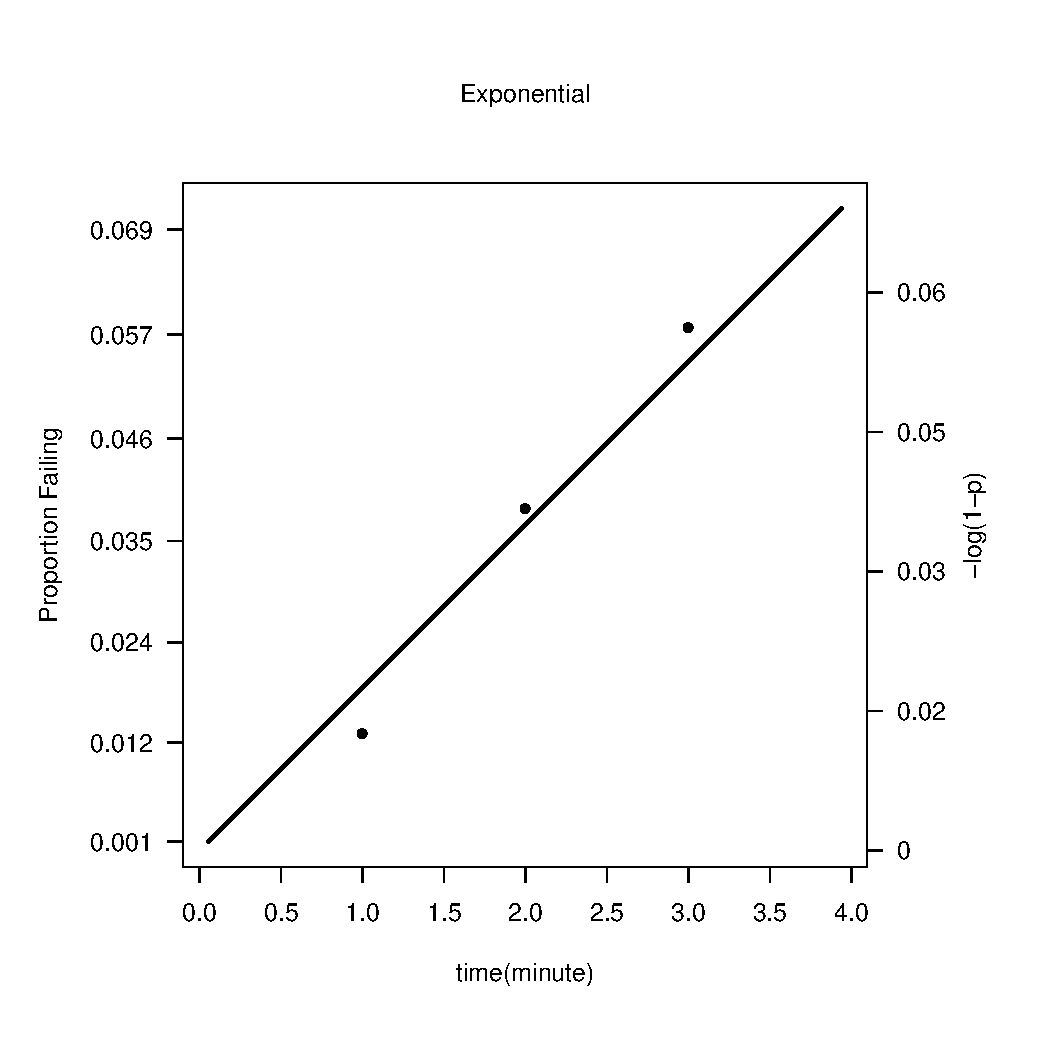
\includegraphics[width = .5\textwidth]{fig_8_2_a.pdf}
			\includegraphics[width = .5\textwidth]{fig_8_2_b.pdf}
	\item[(c)]	Both of the log-likelihood of the two distributions are -54.8, thus there are no difference between them.
\end{itemize}

%----------------------------------------------------------------------------------------
%	8.3
%----------------------------------------------------------------------------------------
8.3 	
\begin{itemize}
\item[]
	By the equation (8.3), we perform a likelihood-ratio test.
	$$H_0: (\beta, \eta)=(\beta_0, \eta_0)\ \ ;\ \ H_1: (\beta, \eta)\neq(\beta_0, \eta_0) $$
	 If $$-2log\left[ \frac{L(\beta_0, \eta_0)}{L(\widehat{\beta}_0, \widehat{\eta}_0)} \right]>\chi_{1-\alpha, 2}^2$$
	than, $H_0$ would be rejected. Under the condition of the null hypothesis, the likelihood ratio would be
	$$-2log\left\{ \frac{\prod_{i = 1}^3\left[ \left( 1- e^{-\left(\frac{t_i}{\widehat{\eta}\prime}\right)} \right) - \left( 1- e^{-\left(\frac{t_{i-1}}{\widehat{\eta}\prime} \right)} \right) \right]^{l_i}  \prod_{j = 1}^3\left[ e^{-\left(\frac{t_j}{\widehat{\eta}\prime} \right)} \right]^{l_j}}{\prod_{i = 1}^3\left[ \left( 1- e^{-\left(\frac{t_i}{\widehat{\eta}}\right)^{\widehat{\beta}}} \right) - \left( 1- e^{-\left(\frac{t_{i-1}}{\widehat{\eta}} \right)^{\widehat{\beta}}} \right) \right]^{l_i}  \prod_{j = 1}^3\left[ e^{-\left(\frac{t_j}{\widehat{\eta}} \right)^{\widehat{\beta}}} \right]^{l_j}} \right\} = 0.7232654$$, where $\widehat{\beta}$ and $\widehat{\eta}$ are the mle of parameters of Weibull distribution and $\widehat{\eta}$ is the mle of parameters of exponential distribution. Let $\alpha = 0.05$, $\chi_{1-\alpha, 2}^2 = \chi_{0.95, 2}^2 = 5.9915$. Hence, $H_0$ is not rejected.
\end{itemize}

\newpage
%----------------------------------------------------------------------------------------
%	8.4
%----------------------------------------------------------------------------------------
8.4 	
\begin{itemize}
	\item[(a)]	Based on $Z_{\widehat{F}(2)} \sim N(0, 1)$, the $95\%$ C.I. is  $$\left[\widehat{F}(2) \pm z_{1-\frac{0.05}{2}}\widehat{se}_{\widehat{F}(2)} \right].$$ $$\widehat{F}(2) = 1-e^{-e^{\frac{log2 - 3.162}{0.743}}} = 0.035 \text{, where} \ \widehat{\mu}_{mle} = 3.162\ \text{and}\ \widehat{\sigma}_{mle} = 0.743$$ By equation $(8.10)$, $$ \widehat{se}_{\widehat{F}(2)} = \sqrt{\left( \frac{\partial F(2)}{\partial \mu} \right)^2\widehat{Var}\left(\widehat{\mu}\right) + 2\left( \frac{\partial F(2)}{\partial \mu} \right)\left( \frac{\partial F(2)}{\partial \sigma} \right)\widehat{Cov}\left(\widehat{\mu}, \widehat{\sigma} \right) + \left( \frac{\partial F(2)}{\partial \sigma} \right)^2\widehat{Var}\left(\widehat{\sigma}\right)}, $$  $\widehat{se}_{\widehat{F}(2)} = 0.011$. Thus, $[0.014, 0.056]$ is the $95\%$ C.I.
	\item[(b)]	Based on $Z_{logit} \sim N(0, 1)$, $$\left[\frac{\widehat{F}(2)}{\widehat{F}(2) + \left(1-\widehat{F}(2) \right)w},  \frac{\widehat{F}(2)}{\widehat{F}(2) + \frac{1-\widehat{F}(2) }{w}}\right], $$ where $$w = e^{z_{1-\frac{0.05}{2}}\frac{\widehat{se}_{\widehat{F}(2)}}{\widehat{F}(2)\left( 1-\widehat{F}(2) \right)}} = 1.847\ \ . $$ Thus, $[0.019, 0.063]$ is  the $95\%$ C.I. of $F(2)$.  
	\item[(c)]	The confidence interval based on $Z_{\widehat{F}(2)} \sim N(0, 1)$ is thinner than the other on under the same level.
\end{itemize}

%----------------------------------------------------------------------------------------
%	9.3
%----------------------------------------------------------------------------------------
9.3 	
\begin{itemize}
	\item[(a)]	and\ \  (b) $$\widehat{\mu}^* = 10.3901 \text{\ \ and\ \ } \widehat{\sigma}^* = 0.3460$$
	\item[(c)]	$$\widehat{\mu} = 10.2299 \text{\ \ and\ \ } \widehat{\sigma} = 0.3164$$ 
			$$Z_{log\left( \widehat{t}_{0.1}^* \right)} = \frac{log\left( \widehat{t}_{0.1}^* \right) - log\left( \widehat{t}_{0.1} \right)}{\widehat{se}_{log\left( \widehat{t}_{0.1}^* \right)}}$$
			$$\widehat{t}_{0.1} = e^{\widehat{\mu} + \widehat{\sigma}\Phi_{sev}^{-1}(0.1)} \text{\ \ and \ \ } \widehat{t}_{0.1}^* = e^{\widehat{\mu}^* + \widehat{\sigma}^*\Phi_{sev}^{-1}(0.1)}$$
			$$log\left( \widehat{t}_{0.1} \right) = \widehat{\mu} + \widehat{\sigma}\Phi_{sev}^{-1}(0.1)=9.518 \text{\ \ and\ \ }log\left( \widehat{t}_{0.1}^* \right) = \widehat{\mu}^* + \widehat{\sigma}^*\Phi_{sev}^{-1}(0.1)=9.611 $$
			$$\widehat{se}_{log\left( \widehat{t}_{0.1}^* \right)} = \frac{\widehat{se}_{ \widehat{t}_{0.1}^* }}{\widehat{t}_{0.1}^* }$$
			, where $\widehat{se}_{ \widehat{t}_{0.1}^* }$ can be calculated by equation (8.10).
	\item[(d)]	and\ \  (e)\ \\
			\includegraphics[width = 0.65\textwidth]{fig_9_3_de.png}\\
			The $95\%$ C.I. of $t_{0.1}$ is $[8472.97, 17252.16]$ which differs from the C.I. in table 9.2 for the condition in this problem based on resampling from the original data.
\end{itemize}

%------------------------------------------------
\end{document}